\documentclass[12pt,twocolumn]{article}  % Change to report, book, etc. if needed

% Essential Packages
\usepackage[utf8]{inputenc}   % Handle UTF-8 encoding
\usepackage[T1]{fontenc}      % Proper font encoding
\usepackage{lmodern}          % Modern font
\usepackage{geometry}         % Page margins
\geometry{margin=1in}        % Set 1-inch margins

% Math and Symbols
\usepackage{amsmath, amssymb} % Math symbols and environments
\usepackage{physics}          % Common physics notation
\usepackage{siunitx}          % SI unit formatting

% Graphics and Figures
\usepackage{graphicx}         % Image inclusion
\usepackage[font=tiny]{caption, subcaption} % Better figure captions
\usepackage{float}            % Control float positioning
\usepackage{listings}
\usepackage{color}

\lstset{language=Python}
\definecolor{dkgreen}{rgb}{0,0.6,0}
\definecolor{gray}{rgb}{0.5,0.5,0.5}
\definecolor{mauve}{rgb}{0.58,0,0.82}

\lstset{frame=top,
  language=Python,
  aboveskip=3mm,
  belowskip=3mm,
  showstringspaces=false,
  columns=flexible,
  basicstyle={\scriptsize\ttfamily},
  numbers=none,
  numberstyle=\tiny\color{gray},
  keywordstyle=\color{blue},
  commentstyle=\color{dkgreen},
  stringstyle=\color{mauve},
  breaklines=true,
  breakatwhitespace=true,
  tabsize=3
}


% Tables
\usepackage{booktabs}         % Better table formatting
\usepackage{array}            % Extended table options



% Title and Author
\title{Spacecraft Mission}
\author{Alex Freeman}
\date{\today}

\begin{document}

\maketitle


This report will cover all parts of assignment one in the Aerospace 720 course

\section{Orbital Propagation}

\subsection{Solving Kepler's Equation}

\textbf{I)} We need to solve Kepler's Equation using numerical methods. Using the Newton-Rasphon Method we can take the eccentricity and mean anamoly as 
inputs and numerically solve for the eccentric anamoly. 

\begin{lstlisting}
def Kepler(e, M, tol = 1e-12, max_i = 1000):
    E = M                               # Guess solution
    for i in range(max_i):
        f_E = E - e * np.sin(E) - M     # Define the function in terms of f(E) = 0
         f_prime = 1 - e * np.cos(E)    # Derive the function in terms of E
        del_E = f_E / f_prime           
        E_new = E - del_E               # Calculate the new eccentric anamoly
        if np.abs(del_E) < tol:         # If the value is within the set tolerance 
            theta = 2*np.arctan(np.tan(E_new/2) * ((1+e)/(1-e))**(0.5))
            return theta                # Return true anamoly
        E = E_new
\end{lstlisting}
\vspace{0.5cm}
\noindent \textbf{II)} If we set the tolerance to $1e-12$, we can compute the true anamoly of the asteroid 
at $t_0$ and $t_0 + 100$ days. A\_ae0 is the OBJ data of the asteroid, it is an array.
\begin{lstlisting}
trueAnamoly_asteroidt_0 = Kepler(A_ae0[2], A_ae0[6])  
meanAnamolyt_100 = get_mean_anamoly(100*(3600*24), A_ae0[6], A_ae0[1])
trueAnamoly_asteroidt_100 = Kepler(A_ae0[2], meanAnamolyt_100)
\end{lstlisting}
Printing these values gives that the true anamoly $\theta_{t_0} = 1.4246$ and $\theta_{t_0 + 100} = 2.1369$. 
Where these answers are in radians.

\vspace{0.5cm}
\noindent \textbf{III)} Now I have created a function that takes in a state of orbital elements and returns 
the position and velocity vectors at that point. It uses a rotation matrix to convert from 
the perifocal frame to the ECI frame. This is defined via $i, \omega$, and $\Omega$ terms and is 
calculated using the defind matricies in the appendix.
\begin{lstlisting}   
def COE2RV(arr, mu):
    a, e, i, Omega, omega, theta_var = arr[0:6]
    h = np.sqrt(mu * a * (1 - e**2))
    r = a*(1-(e**2))/(1 + e*np.cos(theta_var))

    arr_r = np.array([r*np.cos(theta_var), r*np.sin(theta_var), 0])
    arr_v = (mu/h)* np.array([-np.sin(theta_var), e + np.cos(theta_var), 0])

    # Rotate position and velocity from perifocal to inertial frame using the 
    # transfomration matrix
    R_matrix = rotation_matrix(i, Omega, omega)

    r_ijk = R_matrix @ arr_r
    v_ijk = R_matrix @ arr_v
    return r_ijk, v_ijk
\end{lstlisting}
\vspace{-0.35cm}
Using this code we can output the state vector at some time $t$. The first three values 
are the $x,y,z$ positions in \textbf{km}. The last three are the velocity values in the $x,y,z$ direction 
in \textbf{km/s}.

\[
\begin{array}{c}
\textbf{At } t_0: \\
\mathbf{\bar{X}} =
\begin{bmatrix}
x = -1.1694365\mathrm{e}{+08} \\
y =  1.53462780\mathrm{e}{+08} \\
z = -6.7446087\mathrm{e}{+06} \\
v_x = -3.1710203\mathrm{e}{+01} \\
v_y = -3.6285380\mathrm{e}{+00} \\
v_z = -1.8931546\mathrm{e}{+00}
\end{bmatrix}
\\[7em] % small vertical space
\textbf{At } t_0 + 100: \\
\mathbf{\bar{X}} =
\begin{bmatrix}
x = -3.2057997\mathrm{e}{+08} \\
y =  6.72659396\mathrm{e}{+07} \\
z = -1.8991445\mathrm{e}{+07} \\
v_x = -1.6964807\mathrm{e}{+01} \\
v_y = -1.2943780\mathrm{e}{+01} \\
v_z = -1.0284663\mathrm{e}{+00}
\end{bmatrix}
\end{array}
\]


\textbf{IV)} Next, I have written a function called "Ephemeris". It returns the position and velocity at some time t.
\begin{lstlisting}
def Ephemeris(t, OBJdata, mu):
    time, a, e, i, Omega, omega, mean_anamoly = OBJdata[0:7]
    nu_t = (mu / (a**3))**0.5
    t = t - t_0_days*days_convert
    mean_anamoly_t = mean_anamoly + nu_t * (t)

    h = np.sqrt(mu * a * (1 - e**2))
    theta_var = Kepler(e, mean_anamoly_t)
    r = a*(1-(e**2))/(1 + e*np.cos(theta_var))
    arr_r = np.array([r*np.cos(theta_var), r*np.sin(theta_var), 0])
    arr_v = (mu/h)* np.array([-np.sin(theta_var), e + np.cos(theta_var), 0])
    R_matrix = rotation_matrix(i, Omega, omega)
    r_ijk = R_matrix @ arr_r
    v_ijk = R_matrix @ arr_v
    
    return r_ijk, v_ijk
\end{lstlisting}

\noindent Using this code we can calculate the position and velocity vectors in the Sun's frame of reference. 


\begin{figure}[H]
    \centering
    \begin{minipage}{0.48\textwidth}
        \centering
        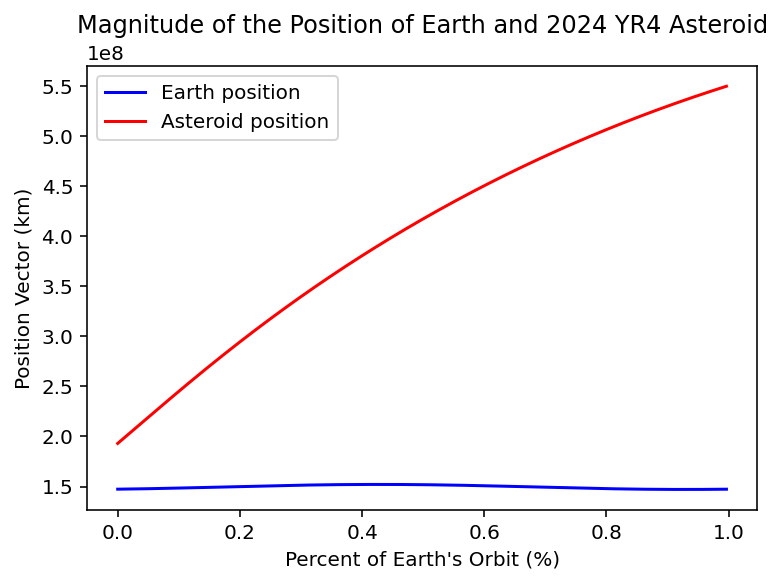
\includegraphics[width=\textwidth]{Images/114-pos.png}
        \caption{Position vectors of Earth and the Asteroid for a full Earth orbital period}
    \end{minipage}
    \hfill
    \begin{minipage}{0.48\textwidth}
        \centering
        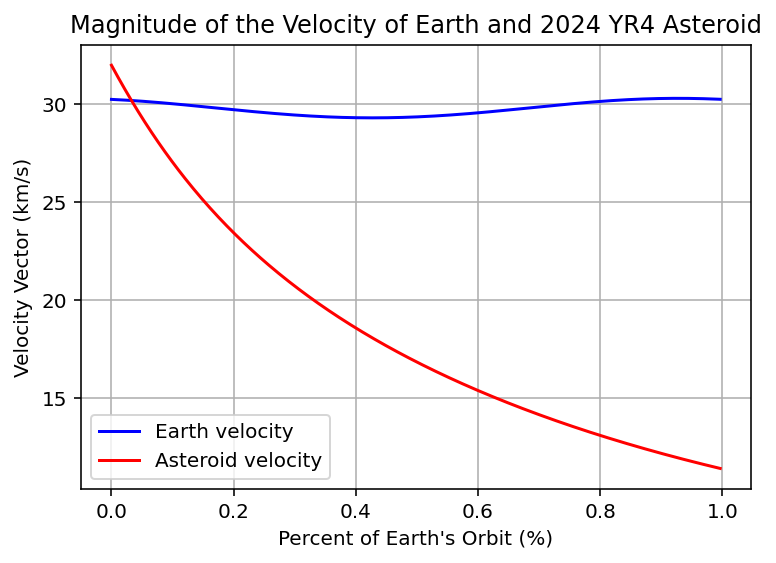
\includegraphics[width=\textwidth]{Images/114-vel.png}
        \caption{Velocity vectors of Earth and the Asteroid for a full Earth orbital period}
    \end{minipage}
\end{figure}
\vspace{-0.2cm}
\noindent Next we can plot the seperation of the two bodies over ten years. Doing this we get the following graph

\begin{figure}[H]
    \centering
    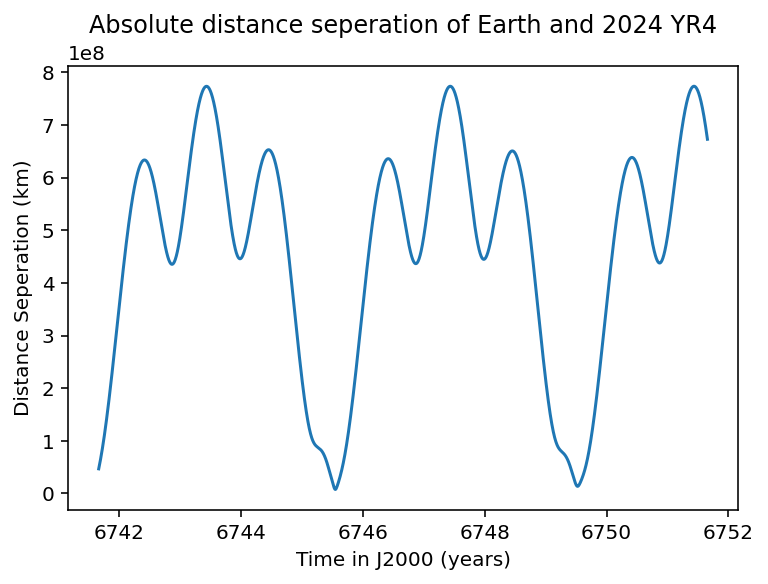
\includegraphics[width=0.48\textwidth]{Images/115-dis.png}
    \caption{Distance between Earth and 2024 YR4 asteroid in kilometers}
\end{figure}

\noindent We can see how the distance is sinusoidal in nature and repeats in an oscillatory fashion. 
This graph shows three distinct peaks, where the middle one is the greatest. We can examine the sydonic period of 
the two bides by examing the equation of the two periods $\frac{1}{T_{syd}} = |\frac{1}{T_{Earth}} - \frac{1}{T_{Asteroid}}|$. And using the orbital periods,
we can see that roughly every 1.33 years, the two bodies are at their closest approach. This lines up well with the graph produced,
showing the magnitude in their seperation. 


\subsection{Numerical Integration}
To derive the necessary state function we have:
\begin{equation}
    \ddot{\mathbf{r}} = -\frac{\mu}{r^3} \mathbf{r}
\end{equation}
From here we know that $\frac{dv}{dt} = \dot{r}$ giving:
\begin{equation}
    \frac{d\mathbf{v}}{dt} = -\frac{\mu}{r^3} \mathbf{r}
\end{equation}
Expanding each vector as three-dimensional components in $x,y,z$:

\begin{equation}
    \frac{dx}{dt} = v_{x},  \frac{dy}{dt} = v_{y},   \frac{dz}{dt} = v_{z}
\end{equation}


\begin{equation}
    \frac{dv_{x}}{dt} = -\frac{\mu}{r^3} x, \frac{dv_{y}}{dt} = -\frac{\mu}{r^3} y, \frac{dv_{z}}{dt} = -\frac{\mu}{r^3} z
\end{equation}
Where $r = \sqrt{x^{2} + y^{2} + z^{2}}$
\newline
We can now define a state vector $\mathbf{\bar{X}}$


\begin{equation}
    \mathbf{\bar{X}} = 
    \begin{bmatrix}
        x \\
        y \\
        z \\
        v_x \\
        v_y \\
        v_z
        \end{bmatrix}
\end{equation}

Finally, deriving this state vector gives the following:

\begin{equation}
    \mathbf{\dot{\bar{X}}} = 
    \begin{bmatrix}
        v_x \\
        v_y \\
        v_z \\
        -\frac{\mu}{r^3} x \\
        -\frac{\mu}{r^3} y \\
        -\frac{\mu}{r^3} z
        \end{bmatrix}
\end{equation}
Now we can use a function to define the right-hand side of this equation
\begin{lstlisting}
def TBP_ECI(t, state_X, mu):
    x, y, z, vx, vy, vz = state_X  # Unpack state vector
    r = np.sqrt(x**2 + y**2 + z**2)  # Compute radius
    ax, ay, az = -mu * x / r**3, -mu * y / r**3, -mu * z / r**3  # Acceleration components
    return [vx, vy, vz, ax, ay, az]  # Return derivatives
\end{lstlisting}
With this function we can use $SciPy's$ integration feature with solve\_ivp. We can pass 
through a set of initial conditions: a position and velocity vector. It passes through the 
gravitational parameter, $\mu$ as an argument when solving the differential system. Furthermore, 
it uses the Runge-Kutta 45 method to integrate. 
\begin{lstlisting}
r0 = np.linalg.norm(X0[:3])  # Initial distance from Earth's center (km)
v0 = np.linalg.norm(X0[3:])  # Initial speed (km/s)
a = 1/(2/r0 - v0**2/mu_earth)  # Semi-major axis (km)
T = 2 * np.pi * np.sqrt(a**3/mu_earth)  # Orbital period (s)

# Set integration time span for two orbital periods
t_start = 0
t_end = 2 * T  # Two orbital periods
time_step = 10  # Output every 10 seconds
t_eval = np.arange(t_start, t_end, time_step)  

# Solve the system using solve_ivp with strict tolerances
solution = solve_ivp(
    TBP_ECI, (t_start, t_end), X0, t_eval=t_eval, method='RK45',
    args=(mu_earth,), rtol=1e-12, atol=1e-12
)

# Extract components
x, y, z = solution.y[0], solution.y[1], solution.y[2]
vx, vy, vz = solution.y[3], solution.y[4], solution.y[5]
\end{lstlisting}


\begin{figure}[H]
    \centering
    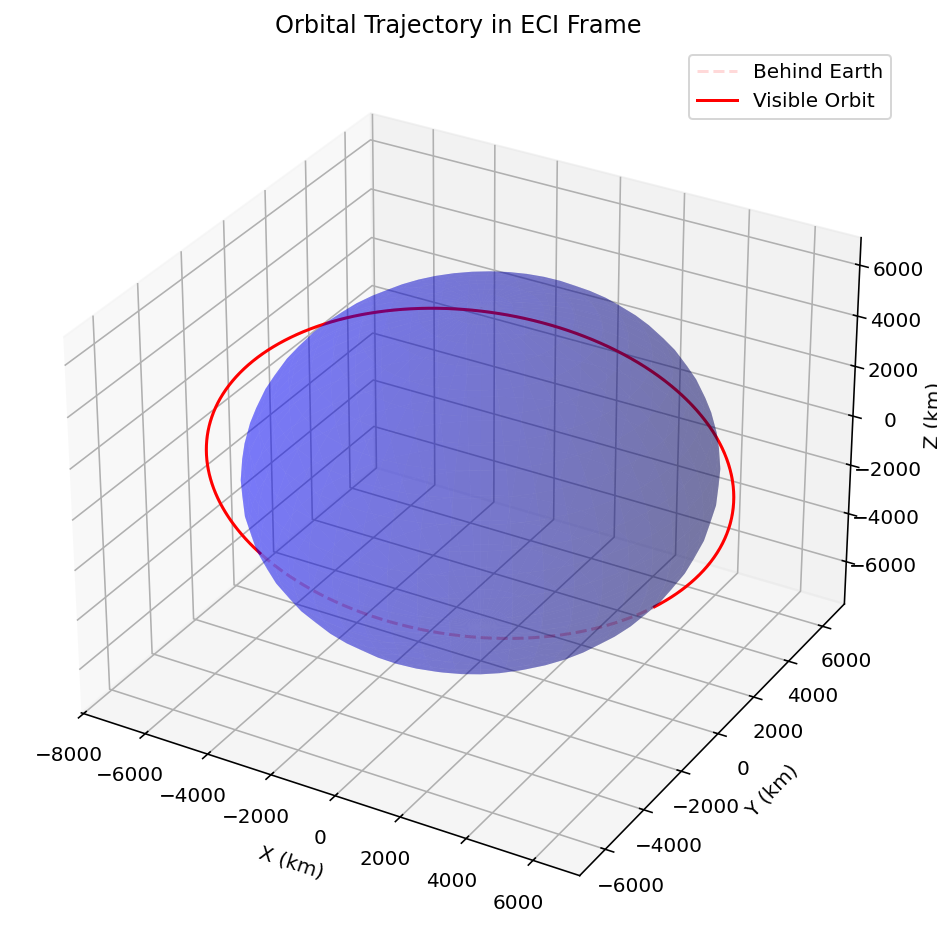
\includegraphics[width=0.48\textwidth]{Images/123-3d.png}
    \caption{Orbital trajectory in ECI frame with initial conditions given from $X_0$}
\end{figure}

\begin{figure}[H]
    \centering
    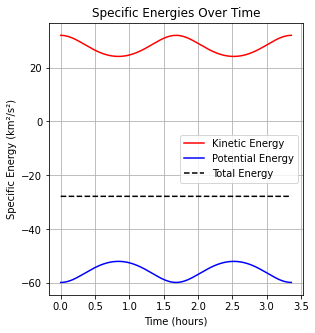
\includegraphics[width=0.4\textwidth]{Images/124-energies.png}
    \caption{How Kinetic, Potential, and Total energies change throughout the orbit }
\end{figure}

This graph shows the sinusoidal nature of the different specific energies. Importantly, we can see how the 
kinetic and potential energies always sum to the same value. This ensures that the total energy remains constant, which we would expect 
as this is a closed system with no external forces. 

\begin{figure}[H]
    \centering
    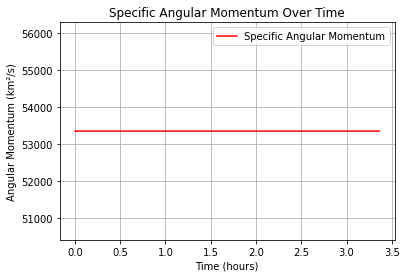
\includegraphics[width=0.48\textwidth]{Images/124-L.png}
    \caption{Graph shows the change in the angular momentum over the orbit is zero}
\end{figure}
\noindent Here we see this graph depicting how the angular momentum changes over time. It shows how the angular momentum stays 
at a constant value and remains constant. This makes sense because the angular momentum is defined as the cross product
between the position and velocity vector.
\setcounter{equation}{0}
\begin{equation}
\frac{dh}{dt} = \frac{d}{dt}(\bar{r} \times \dot{\bar{r}}) \implies \frac{dh}{dt} = \bar{r} \times \frac{d\dot{\bar{r}}}{dt}
\end{equation}

\begin{equation}
\frac{dh}{dt} = \bar{r} \times -\frac{\mu}{r^{3}}\bar{r} \implies \frac{dh}{dt} = 0
\end{equation}
\vspace{0.2cm}

So yes, these diagrams make physical sense, based upon the conservation laws of both Energy and Angular Momentum


\section{Orbital maneuvers and mission design}
\subsection{Reachability Analysis}

\begin{lstlisting}
def RV2COE(state_x, mu):
    r_vec = state_x[0:3]
    v_vec = state_x[3:6]
    r_mag = norm(r_vec)
    v_mag = norm(v_vec)
    
    a = r_mag / (2 - (r_mag*v_mag**2/mu))
    h = np.cross(r_vec, v_vec)
    h_mag = norm(h)
    e_vec = np.cross(v_vec, h) / mu - r_vec / r_mag
    e_mag = norm(e_vec)
    i = np.arccos(h[2]/h_mag)
    
    n_vec = np.cross(k_hat, h)
    n_mag = norm(n_vec)
    n_hat = n_vec / n_mag
    Omega_raan = np.arccos(n_hat[0])
    if n_hat[1] < 0:
        Omega_raan = 2*np.pi - Omega_raan
    
    omega = np.arccos(np.dot(n_vec, e_vec)/(n_mag * e_mag))
    if e_vec[2] < 0:
        omega = 2*np.pi - omega
        
    cos_theta = np.dot(r_vec, e_vec) / (r_mag * e_mag)
    cos_theta = np.clip(cos_theta, -1.0, 1.0)  
    theta = np.arccos(cos_theta)
    if np.dot(r_vec, v_vec) < 0:
        theta = 2*np.pi - theta
    
    return np.array([a, e_mag, i, Omega_raan, omega, theta])
\end{lstlisting}

Using this function, we can report the COE state for the initial condition. Inputting the vector $\bar{X}$, returns the following elements.

\begin{center}
    \textbf{At } $X_0$:
    COE =
    $\begin{bmatrix}
    a = 7.17813700\mathrm{e}{+03} \\
    e =  7.00000000\mathrm{e}{-02} \\
    i = 1.67551608\mathrm{e}{+00} \\
    \Omega = 3.49065850\mathrm{e}{-01} \\
    \omega = 7.85398163\mathrm{e}{-01} \\
    \theta = 6.28318529\mathrm{e}{+00}
    \end{bmatrix}$  
\end{center}

\begin{lstlisting}
def rotate_matrix(state_x):
    r_vec = state_x[0:3]
    v_vec = state_x[3:6]
    
    r_hat = r_vec/(norm(r_vec))
    

    h_vec = np.cross(r_vec, v_vec)
    h_hat = h_vec / np.linalg.norm(h_vec)  
    t_hat = np.cross(h_hat, r_hat)  

    rotation = np.column_stack((r_hat, t_hat, h_hat))
    
    return rotation
\end{lstlisting}

With this rotation matrix now defined at every point along the orbit, I can define a function named "impulse". This function
takes a rotation matrix, direciton and an initial state as input parameters. It calculates the impulse in the direction of either, 
radius, transverse or normal (which are calculated via 3-D basis vectors). Then the rotation matrix is applied to the impulse to convert
it from the RTN frame to the ECI frame. It adds this vector to the velocity components of the state and then calculates the orbital 
elements of this final state and the inputted initial state to find the difference between components. 
\begin{lstlisting}
def impulse(r_matrix, direct, initial_state):
    dv_ = np.dot(delta_v, direct)

    impulse_eci =  r_matrix @ dv_

    state_final = initial_state.copy()
    state_final[3:] += impulse_eci
    oElements_initial = RV2COE(initial_state, mu_earth)
    oElements_final = RV2COE(state_final, mu_earth)

    coe_diff = oElements_final - oElements_initial

    return coe_diff, oElements_final
\end{lstlisting}

Using these combinations of functions we can apply an impulse in the three different directions and calculate the changes.
\begin{table}[h]
    \centering
    \begin{minipage}{0.48\textwidth} % First table: first three columns
        \centering
        \small
        \setlength{\tabcolsep}{4pt}
        \renewcommand{\arraystretch}{1.1}
        \begin{tabular}{lccc}
        \hline
        Impulse Type & $\Delta a$ & $\Delta e$ & $\Delta i$ \\
        \hline
        Radial     & 0.012927 & $1.28\mathrm{e}{-5}$ & 0 \\
        Transverse & 20.7374  & 0.00267900   & 0 \\
        Normal     & 0.012927 & $1.67\mathrm{e}{-6}$ & $8.85\mathrm{e}{-4}$ \\
        \hline
        \end{tabular}
        \caption{Changes in the semi-major axis, eccentricity and inclination}
    \end{minipage}
    \hfill
    \begin{minipage}{0.48\textwidth} % Second table: last three columns
        \centering
        \small
        \setlength{\tabcolsep}{4pt}
        \renewcommand{\arraystretch}{1.1}
        \begin{tabular}{ccc}
        \hline
        $\Delta \Omega$ & $\Delta \omega$ & $\Delta M$ \\
        \hline
        0 & -0.0191214 & -6.26406 \\
        0 & 0 & 0.0000000149012 \\
        0.000889606 & 0.0000933805 & 0.0000000149012 \\
        \hline
        \end{tabular}
        \caption{Changes in $\Omega$, $\omega$ and mean anamoly}
    \end{minipage}
\end{table}

    

    \begin{figure}[H]
        \centering
    
        % First row
        \begin{subfigure}[t]{0.45\textwidth}
            \centering
            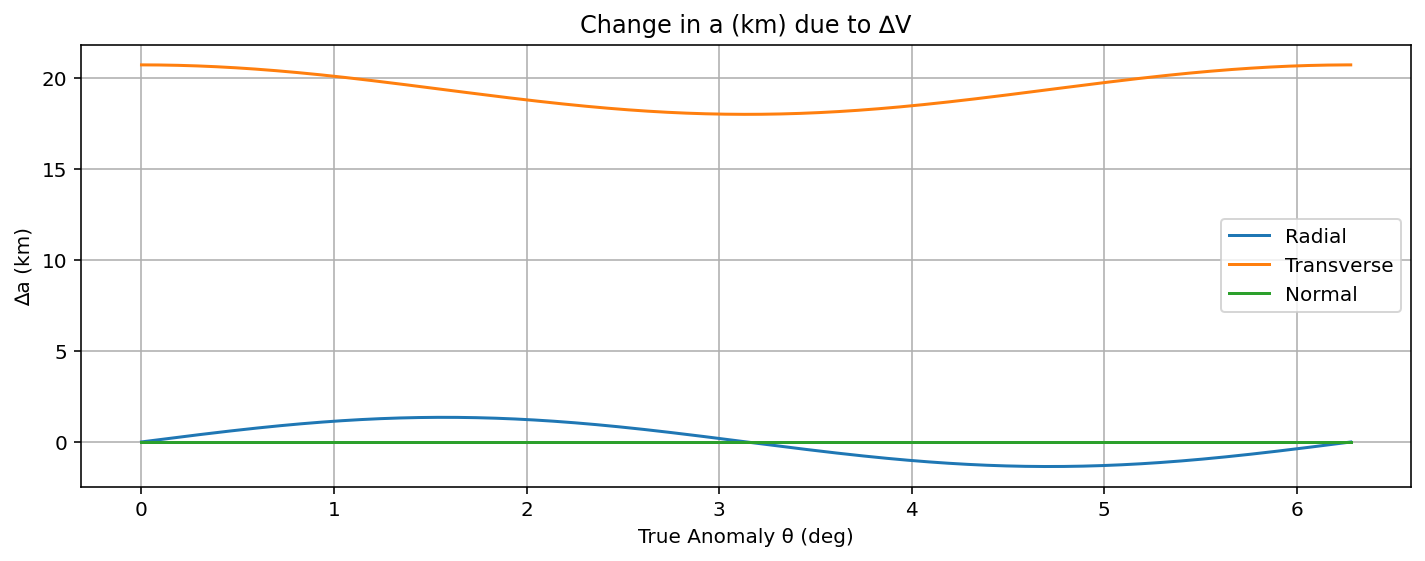
\includegraphics[width=\linewidth]{Images/del_a.png}
            \caption{Graph 1}
        \end{subfigure}
        \hspace{0.05\textwidth}
        \begin{subfigure}[t]{0.45\textwidth}
            \centering
            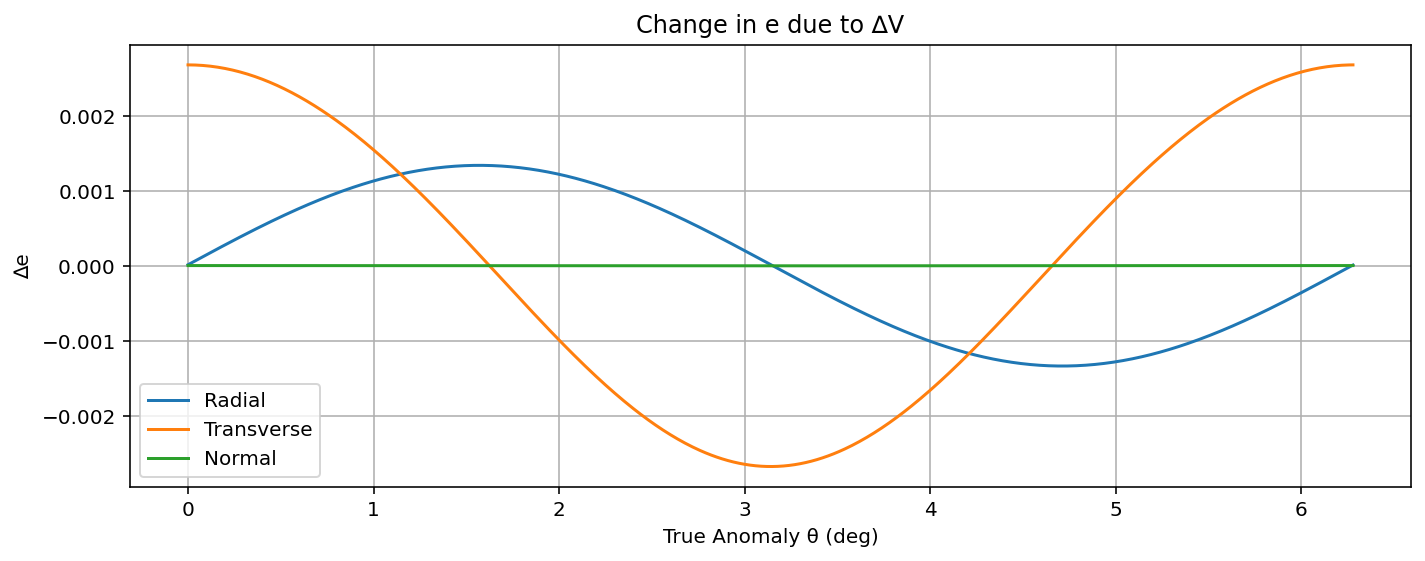
\includegraphics[width=\linewidth]{Images/del_e.png}
            \caption{Graph 2}

        \end{subfigure}
    
        \vspace{1em}
    
        % Second row
        \begin{subfigure}[t]{0.45\textwidth}
            \centering
            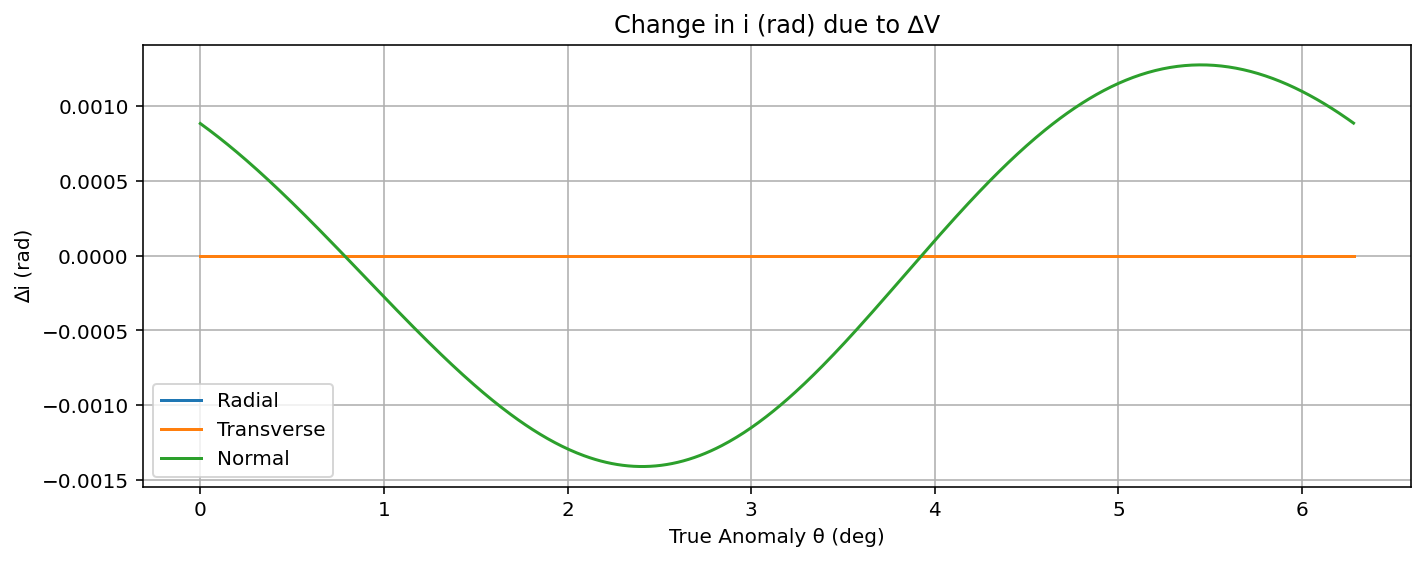
\includegraphics[width=\linewidth]{Images/del_i.png}
            \caption{Graph 3}
        \end{subfigure}
        \hspace{0.05\textwidth}
        \begin{subfigure}[t]{0.45\textwidth}
            \centering
            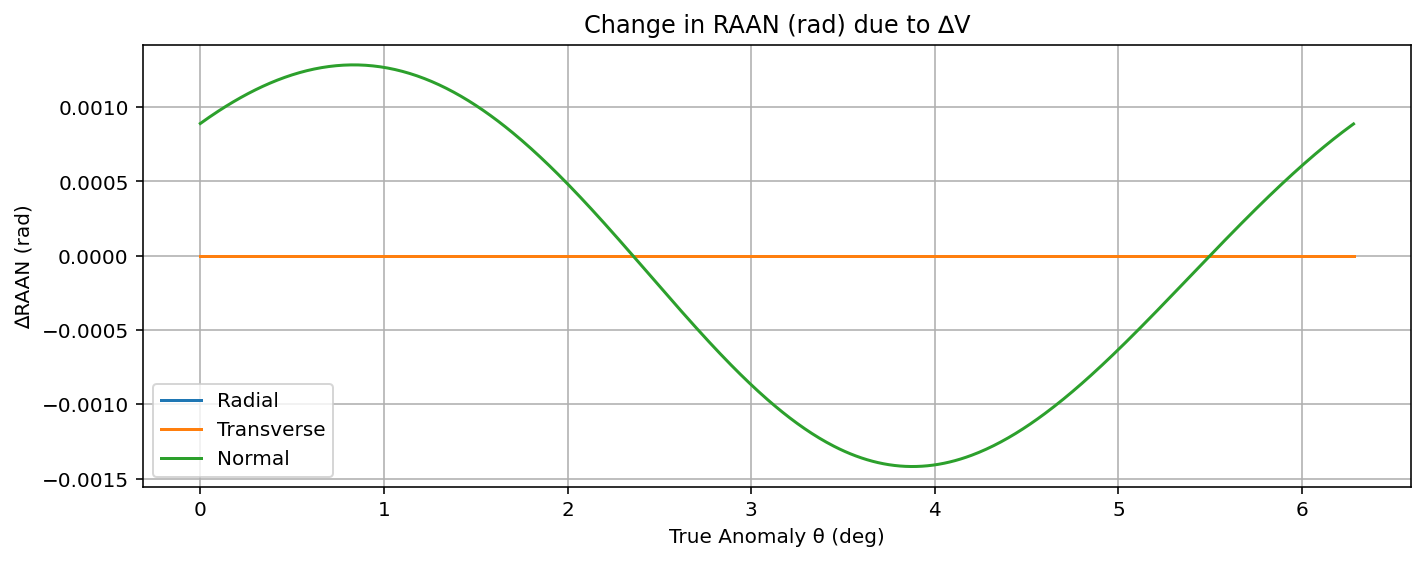
\includegraphics[width=\linewidth]{Images/del_Omega.png}
            \caption{Graph 4}
        \end{subfigure}
    
        \vspace{1em}
    
        % Third row
        \begin{subfigure}[t]{0.45\textwidth}
            \centering
            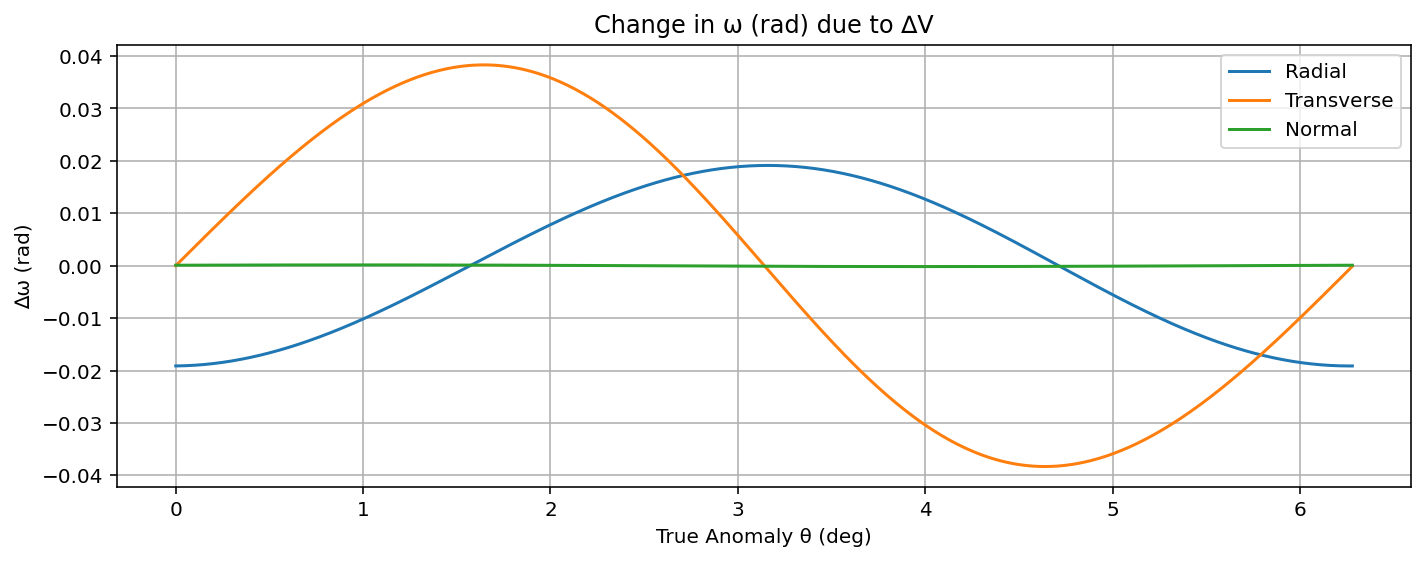
\includegraphics[width=\linewidth]{Images/del_lomega.png}
            \caption{Graph 5}
        \end{subfigure}
        \hspace{0.05\textwidth}
        \begin{subfigure}[t]{0.45\textwidth}
            \centering
            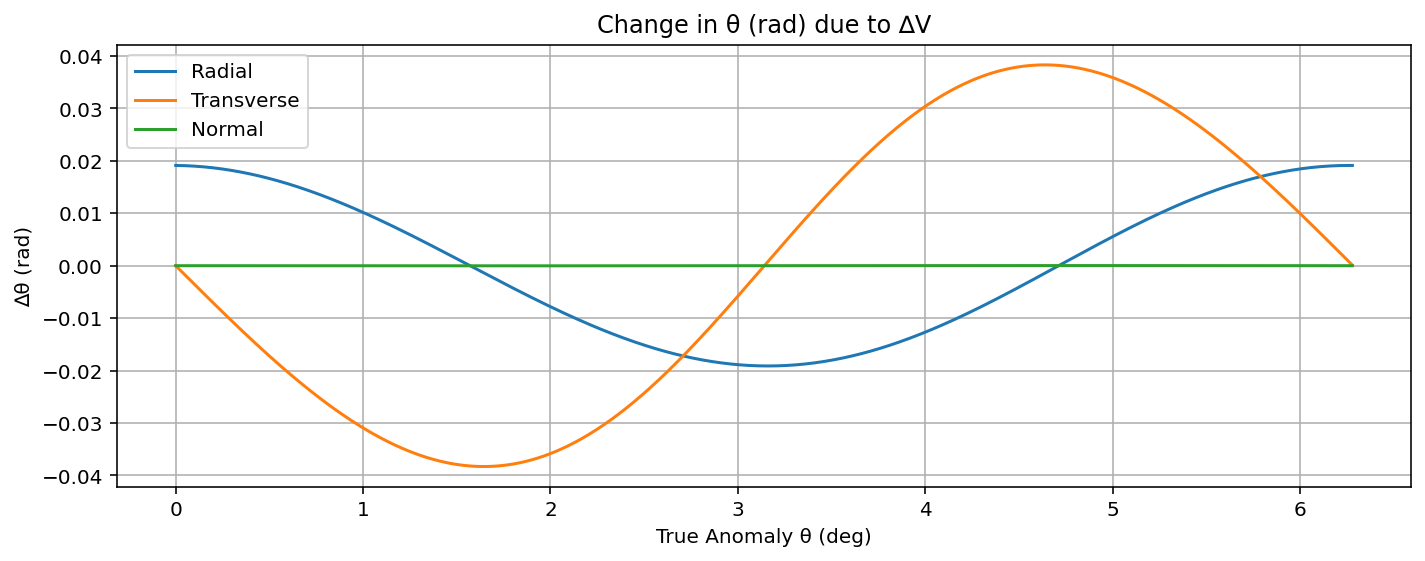
\includegraphics[width=\linewidth]{Images/del_theta.png}
            \caption{Graph 6}
        \end{subfigure}
    
        \caption{Six graphs showing how the classical orbital elements change with impulses}
        \label{fig:six_graphs}
    \end{figure}
Using these graphs we can examine which $\theta$ values maximise $\Delta i$. Using the Signal library apart of Python
and its corrosponding find\_peaks\_cwt function, the peaks of $\Delta i$ are  $-0.0014$ and $0.0013$ radians.
These corrosponding $\theta$ values are $2.36$ and $5.46$ radians. Understanding that the argument of latitude, $u$,
is defined as $\theta + \omega$, and observing that at these theta values, $\omega = 0.79$ and $0.79$ radians.
Hence, $u = 3.145$ and $6.245$ radians. These numbers represent the apogee and perigee respectively (which make sense because the perigee and apogee 
occur at $\pi$ and $2\pi$). Therefore, for maximum change to the inclination, one should provide a normal impulse at the perigee and apogee.

\subsection{Lunar Mission Design}

\noindent Now we can analyse what happens when the apogee of the transfer orbit is increased passed the 
orbital radius of the moon. By increasing this distance 
we are completeing a non-tangential transfer, where the mission will have a lower transfer time, but will arrive
with some non-zero radial velocity.

Using numpy's matrix-oriented math in Python, calculations can be swift looking at the range of apogee values.
\begin{lstlisting}
parking_altitude = 220
parking_radius = parking_altitude + radius_earth

radius_apogee = r_mean*np.arange(1.1, 1.4, 0.01)
semi_major_axis = 0.5*(parking_radius + radius_apogee)
transfer_e = (radius_apogee-parking_radius)/(radius_apogee+parking_radius)
cos_theta_A = (semi_major_axis * (1 - transfer_e**2) / r_mean - 1) / transfer_e
theta_2 = np.arccos(cos_theta_A)
semi_latus_rectum =  semi_major_axis * (1 - transfer_e**2)

v_radial = np.sqrt(mu_earth / semi_latus_rectum) * transfer_e * np.sin(theta_2)
v_transverse = np.sqrt(mu_earth / semi_latus_rectum) * (1 + transfer_e * np.cos(theta_2))
normed_apogee = radius_apogee/r_mean
\end{lstlisting} 

\noindent Now we have the true anamoly, radial, and transverse velocities inside a matrix array for every 
apogee value normalized to the moon's orbital radius. Printing these components, we can see how 
these change as we increase the distance. 
\begin{figure}[H]
    \centering
    \begin{minipage}{0.48\textwidth}
        \centering
        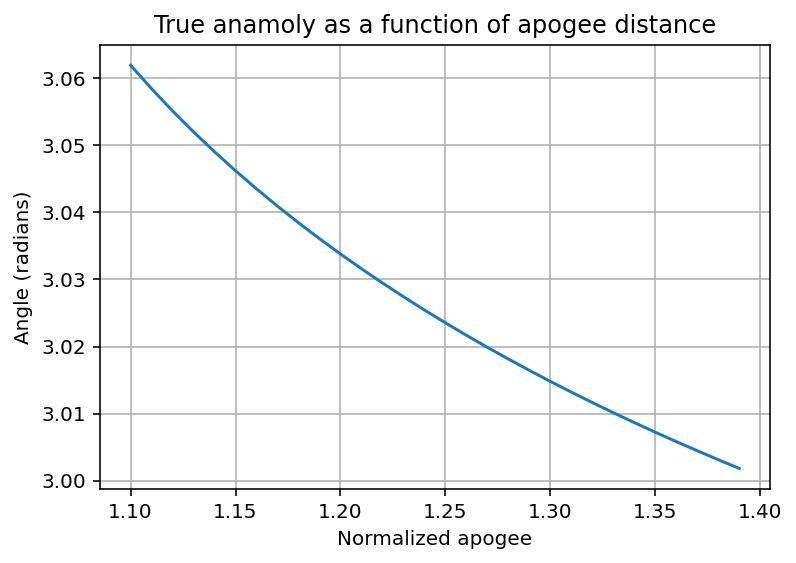
\includegraphics[width=\textwidth]{Images/221-theta.png}
        \caption{Graph depicting how the true anamoly decreases as the apogee distance increases}

    \end{minipage}
    \hfill
    \begin{minipage}{0.48\textwidth}
        \centering
        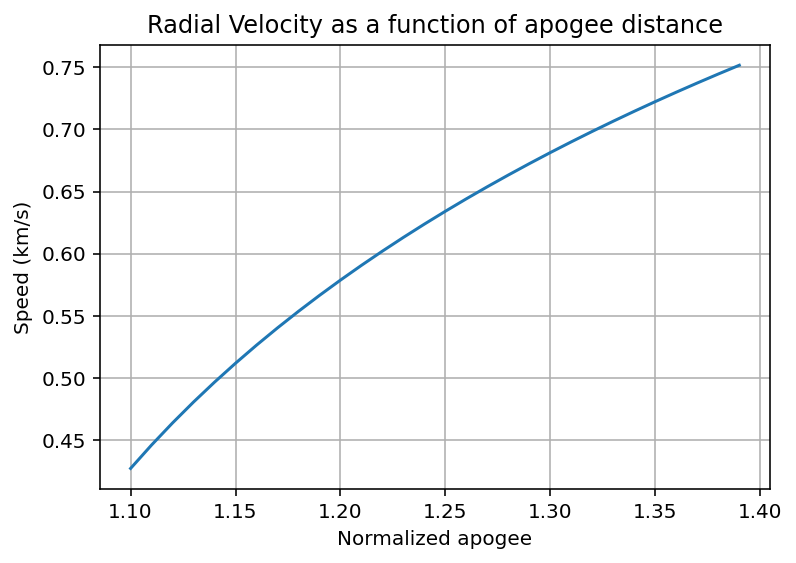
\includegraphics[width=\textwidth]{Images/221-rad.png}
        \caption{Graph depicting how the radial velocity increases as the apogee distance increases}

    \end{minipage}
    \hfill
    \begin{minipage}{0.48\textwidth}
        \centering
        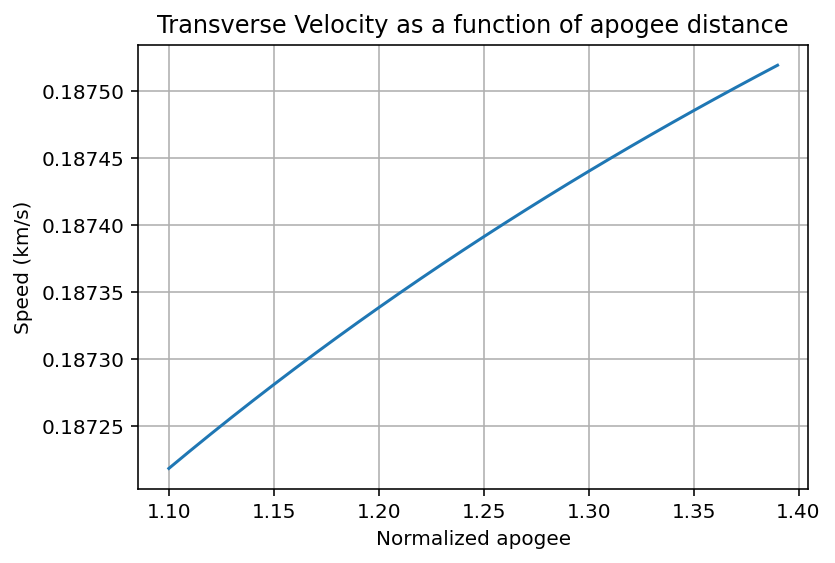
\includegraphics[width=\textwidth]{Images/221-trans.png}
        \caption{Graph depicting how the transverse velocity increases as the apogee distance increases}
    \end{minipage}
\end{figure}

We can see from these figures how the radial component of the velocity 
changes much more significantly that the transverse component.
This is because the radial component is related
 to the orbital energy equation. When the 
semi-major axis is significantly increased, 
to reach beyond the Moon, most of that additional energy 
manifests as radial velocity because it 
directly contributes to increasing the orbital energy and apogee height.
By comparison, the transverse velocity is primarily responsible 
for maintaining orbital angular momentum, so does not change as violently.
\newline
\newline
Next we can observe how the apogee and transfer time are related.
Writing some more code we can examine this, again using numpy's matrix operations.
\begin{lstlisting}
theta_eccentric = 2*np.arctan(np.tan(theta_2/2) * ((1-transfer_e)/(1+transfer_e))**(0.5))
theta_mean = theta_eccentric - transfer_e*np.sin(theta_eccentric)
time_total = time_orbit(semi_major_axis, mu_earth)
delta_t = (time_total / (2 * np.pi)) * theta_mean / days_convert
\end{lstlisting}

This gives the transfer time for every apogee value, which we can plot as the following.

\begin{figure}[H]
    \centering
    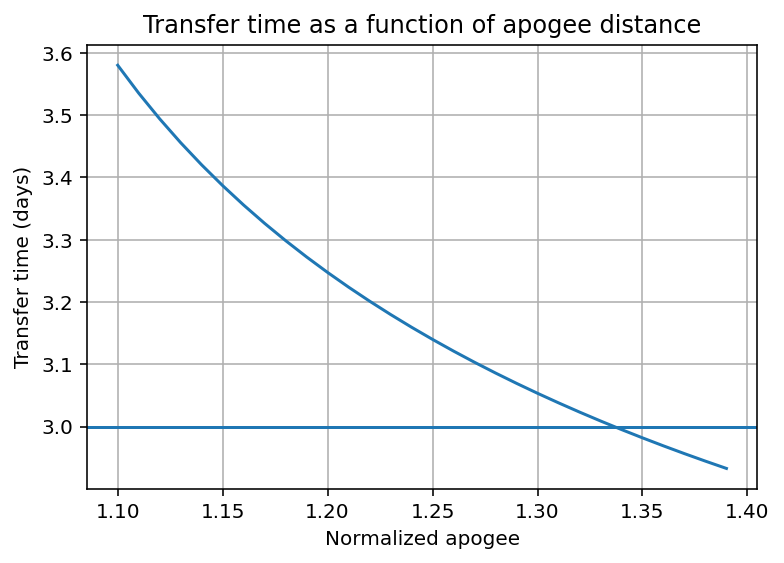
\includegraphics[width=0.48\textwidth]{Images/222-time.png}
    \caption{Graph showing how the transfer time decreases as the apogee value increases}
\end{figure}

This plot clearly shows how the transfer time decreases as the apogee value increases. This makes sense because increasing the 
apogee point, means the spacecraft is intercepting the moon at an earlier stage of its orbit.
There is a horizontal line corrosponding to $t=3$ days. We can look at the intercept of this line with the plot to see that for a 
transfer time of three days, an apogee value of $1.34\cdot r_m$ is required
\begin{figure}[H]
    \centering
    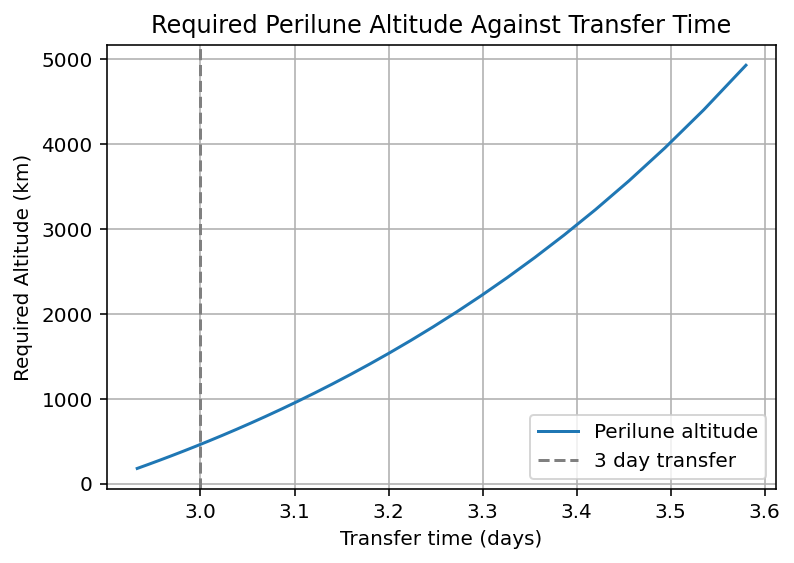
\includegraphics[width=0.48\textwidth]{Images/223-altitude.png}
    \caption{Distance between Earth and 2024 YR4 asteroid in kilometers}
\end{figure}


\onecolumn
\section{Appendix}
   
    

\end{document}
